%\renewcommand{\theequation}{\theenumi}
%\begin{enumerate}[label=\thesection.\arabic*.,ref=\thesection.\theenumi]
%\numberwithin{equation}{enumi}
	
\item {\em Proof: }
%\solution
From Fig. \ref{fig:8.1.28},	
%$\triangle AMC \cong \triangle DMB$  by SAS congruency $\because$
%\begin{enumerate}
%\item $AM = BM$
%\item $CM = DM$
%\item $\phase{AMC}$ = $\phase{DMB}$ ( Vertically Opposite Angles)
%\end{enumerate}
%
%\begin{figure}[!ht]
%\centering
%\resizebox{\columnwidth}{!}{%\documentclass{standalone}
%
%\usepackage{tikz,pgf} %and any other packages or tikzlibraries your picture needs
%
%\begin{document}
%\resizebox{\columnwidth}{!}{
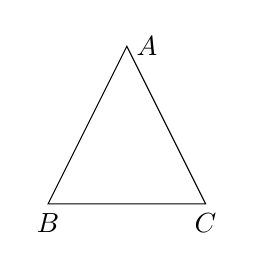
\begin{tikzpicture}
\draw (0,0) node[anchor=north]{$B$}
  -- (1,2) node[anchor=west]{$A$}
  -- (2,0) node[anchor=north]{$C$}
  -- cycle;
\end{tikzpicture}
%}
%\end{document}}
%\caption{}
%\label{fig:8.1.28}	
%\end{figure}
%\item From \eqref{eq:constr_b}, \eqref{eq:constr_c} and \eqref{eq:constr_d},
%%
%%
\begin{align}
\brak{\vec{D}-\vec{B}}^T
\brak{\vec{B}-\vec{C}} &= \myvec{0 & b}\myvec{a \\ 0} = 0
\\
\implies BD \perp BC
\end{align}
%%
%\item From \eqref{eq:constr_a}, \eqref{eq:constr_b}, \eqref{eq:constr_c} and \eqref{eq:constr_d},
\begin{align}
\norm{\vec{A}-\vec{B}} &= \norm{\myvec{-a \\ b}}
\\
\norm{\vec{C}-\vec{D}} &= \norm{\myvec{-a \\ -b}}
\\
\implies \norm{\vec{A}-\vec{B}} &= \norm{\vec{C}-\vec{D}}\\
\text{or, } AB &=CD
\label{eq:solution_abcd}
\end{align}
%%
Noting that BC is the common side, from RHS congruence,  $\triangle ACB \cong  \triangle DCB$.
\subitem  From \eqref{eq:solution_abcd}, noting that $\vec{M}$ is the mid point of both $AB$ and $CD$, 
\begin{align}
CM = \frac{1}{2}CD =\frac{1}{2} AB
\end{align}



%\end{enumerate}
